\chapter{Breve Descrição do Projeto de Formatura}

O projeto de formatura objetiva o desenvolvimento de um sistema de automação residencial completo, com foco na robustez, segurança e facilidade de uso. Para tanto, a modelagem de uma arquitetura flexível, que suportasse os requisitos iniciais, tem papel estrutural no trabalho. A plataforma do sistema é enfática em sua proposta de camadas, onde integração entre os níveis é feito por meio de troca de mensagens, utilizando a infraestrutura de comunicação desenvolvida. No decorrer desta monografia, serão apresentados os pontos essenciais do projeto, bem como a descrição das soluções adotadas.

\subsection{Hardware}

\subsection{Software}

As partes de software do sistema são divididas de acordo com a sua aplicação, localização e uso. Neste momento, serão considerados somente os softwares de aplicação, de maneira que todo o software de operação do hardware está descrito na no item (MARCAR ITEM).

Em contato mais próximo dos dispositivos de hardware está o servidor local, Morpheus. O servidor local é responsável pela interconexão dos módulos da casa com os serviços de nuvem disponíveis. A troca de informação entre os módulos físicos e o Morpheus é realizada por meio de mensagens, codificadas em um protocolo desenvolvido pelo grupo, e encaminhadas por meio do protocolo MQTT, com um broker local disponível na residência. O envio de mensagens é feito em tópicos, aos quais o módulo pode publicar ou se inscrever, mas de acordo com o seu serial number, de modo a evitar que um módulo consiga ter acesso ao canal de outro módulo. O servidor local, no entanto, precisa de um certificado válido para que possa se inscrever no seu canal, onde a troca de mensagens é realizada com criptografia assíncrona. Quando a mensagem chega nesse servidor, ela é convertida em um formato intermediário e colocada em um fila de entrada, onde uma thread de um pool irá retirá-la para efetuar o processamento, e conversão para um JSON esperado pela nuvem.

A segunda transmissão de dados, entre o Morpheus e os serviços de nuvem é feita por meio de um canal WebSocket, onde a conexão permanece ativa a todo o momento. Os serviços de nuvem tratam a chegada da mensagem, e interagem com um cliente web, por meio de um dashboard, sobre o qual o usuário pode interagir.

Para que a robustez do sistema seja assegurada, o projeto também conta com um sistema emergencial, no caso de não haver internet na casa, ou qualquer problema com o servidor local. O usuário pode se conectar diretamente na rede de um dos módulos, sem a integração com a nuvem.


\subsection{Bases de Dados}

\subsection{Redes e Conectividade}

A interconectividade local, fruto da infraestrutura de comunicação disponível, é feita por meio de ondas de rádio, na frequência comercial relativa às redes WiFi. Cada um dos módulos possui um microcontrolador e radio transmissor ESP8266, o qual se conecta à rede da residência, e envia mensagens para o respectivo tópico. Os módulos possuem tópicos específicos, finalizados em m2s, module to  server, e no seu caminho há o serial ID do módulo em questão. Essa garantia é feita por meio de configurações no broker, onde assegura-se que o endereço do tópico possui as credenciais do módulo autenticado.
O servidor local possui um tópico específico, finalizado em s2m, server to module, e tem acesso de subscrição a todos os tópicos relativos às publicações de módulos. A autenticação do servidor, ao contrário dos módulos, é feito por meio de certificados digitais, e há criptografia assíncrona na camada de transporte (SSL).

Para a intercomunicação entre a casa e a nuvem, houve uma mudança na arquitetura inicial proposta. De início o projeto estabelecia que o servidor local também tivesse a responsabilidade de ser um servidor para requisições externas, oferecendo para isso uma API Rest. Entretanto, os impactos dessa decisão afetam enormemente a segurança, já que a casa estaria suscetível a ataques de negação de serviço (DoS). Assim, posteriormente foi optado por uma mudança e a utilização de WebSockets na construção, de modo que a conexão permanece ativa, e a responsabilidade por se proteger de ataque do tipo concentra-se na nuvem, onde há uma infraestrutura muito mais robusta e a possibilidade de uso de serviços de terceiros, como servidores Akamai.

Em alto nível, é representado na \autoref{fig:arquiteturaHedwig} o diagrama arquitetural do projeto e, na \autoref{fig:diagramaDeComunicacao} é disponibilizada a arquitetura do servidor local (Morpheus) e a sua conectividade com a nuvem e módulos.

\begin{figure}[htb]
	\caption{\label{fig:arquiteturaHedwig}Diagrama Arquitetural}
	\begin{center}
	    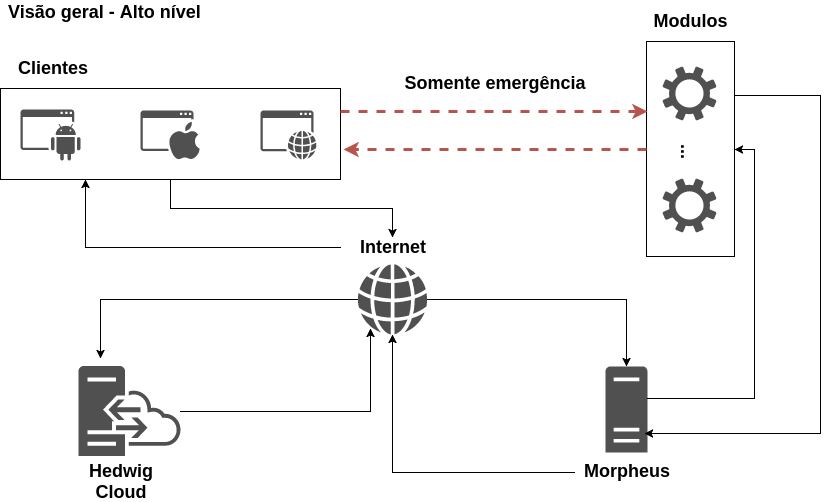
\includegraphics[scale=0.5]{arquiteturaHedwig}
	\end{center}
	\legend{Fonte: os autores}
\end{figure}

\begin{figure}[htb]
	\caption{\label{fig:diagramaDeComunicacao}Diagrama de Comunicação}
	\begin{center}
	    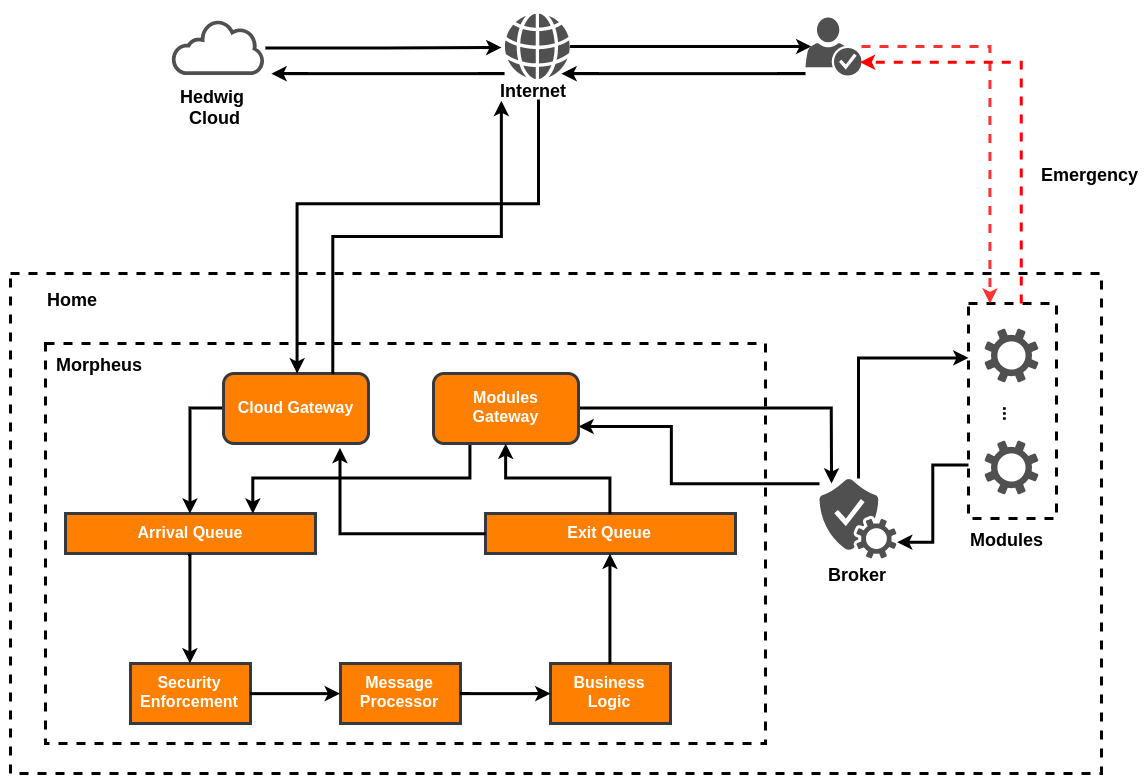
\includegraphics[scale=0.4]{diagramaDeComunicacao}
	\end{center}
	\legend{Fonte: os autores}
\end{figure}